\section{Palabras de estructura triplicada (I)}

%----------
% MT-5A
%----------

\subsection{MT Multicinta Determinista}

\subsubsection*{Diseño propuesto}
El algoritmo de resolución es el siguiente:

\begin{enumerate}
    \item Leer \texttt{a} o \texttt{b} en la cinta 0 tres veces, y poner un \texttt{1} en la cinta 1.
    \item Si no es el final de la cinta, volver al paso anterior. En caso afirmativo, tendremos en la cinta 1 el tamaño de la palabra $w = n/3$, en base uno.
    \item Por cada \texttt{1} en la cinta 1:
    \begin{enumerate}[1.]
        \item Copiar la letra de la cinta 0 a la cinta 1, y borrarla de la cinta 0, sobreescribiendo los \texttt{1} y moviendo a la izquierda ambas cintas.
    \end{enumerate}
    \item Por cada letra de la cinta 1:
    \begin{enumerate}[1.]
        \item Validar que las letras de ambas cintas son iguales, mover la cinta 0 a la izquierda, borrando las letras, y la cinta 1 a la derecha.
    \end{enumerate}
    \item Por cada letra de la cinta 1:
    \begin{enumerate}[1.]
        \item Validar que las letras de ambas cintas son iguales y mover ambas cintas a la izquierda, borrando las letras.
    \end{enumerate}
    \item Poner un \texttt{1} en la cinta 0 y \textbf{parar}.
\end{enumerate}

El diseño de la máquina queda representado en la Figura \ref{fig:MT-5A}.

\begin{figure}[h]
    \centering
    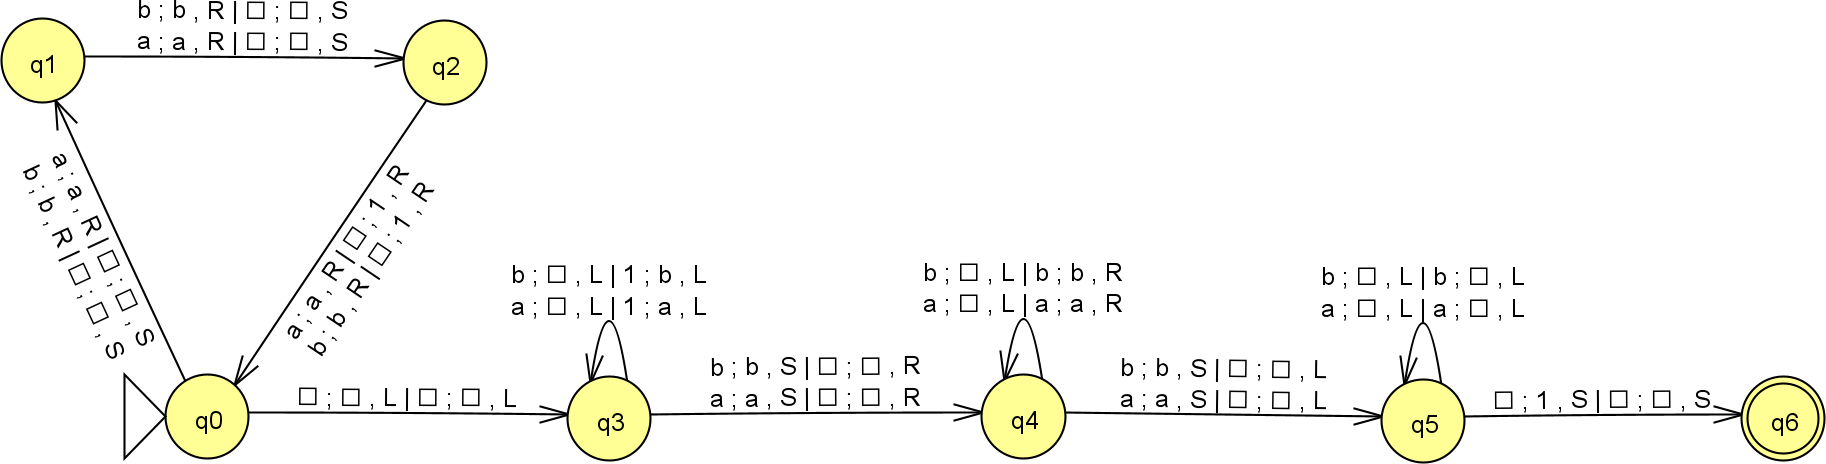
\includegraphics[width=0.8\textwidth]{MT-5A.png}
    \caption{Implementación en JFLAP de MT-5A}
    \label{fig:MT-5A}
\end{figure}


\subsubsection*{Peor caso}
El peor caso es cuando es una palabra de la gramática ($w \cdot w^{-1} \cdot w$), puesto que tiene que comprobarla entera. La estructura de $w$ es irrelevante, puesto que las transiciones no dependen de cómo esté formada.

\subsubsection*{Evaluación empírica}
Realizamos la evaluación empírica en el peor caso, tomando como $n$ el tamaño de la palabra, y midiendo el número de pasos realizados para resolver el problema\footnote{Los datos se pueden encontrar en \texttt{data/MT-5A.csv}.}:

\begin{table}[h]
    \centering
    \begin{tabular}{lcc}
        Entrada & $n$ & Pasos \\
        \hline
        \texttt{aaa}                &  3  & 10 \\
        \texttt{aaaaaa}             &  6  & 16 \\
        \texttt{aaaaaaaaa}          &  9  & 22 \\
        \texttt{aaaaaaaaaaaa}       & 12  & 28 \\
    \end{tabular}
\end{table}

\subsubsection*{Coste computacional}
Para obtener el coste computacional del algoritmo, aplicaremos Diferencias Finitas, basándonos en los datos de la evaluación empírica:

\begin{table}[H]
    \centering
    \begin{tabular}{|l|c|c|c|c|}
        \hline
        $n$ & \textbf{3} & \textbf{6} & \textbf{9} & \textbf{12} \\ \hline
        $T(n)$ & \textbf{10} & \textbf{16} & \textbf{22} & \textbf{28} \\ \hline
        \hline
        $A(n) = T(n) - T(n-2)$ &   & 6 & 6 & 6 \\ \hline
        $B(n) = A(n) - A(n-2)$ &   &   & 0 & 0 \\ \hline
    \end{tabular}
    \label{tab:5A}
\end{table}

Al ser constantes las diferencias finitas primeras, y nulas las segundas, podemos aproximar $T(n)$ con un polinomio de primer orden, es decir, $T(n) = an + b$.\\

Para obtener los valores de $a$ y $b$, usaremos valores de $n$ y $T(n)$ obtenidos en la evaluación empírica:

\begin{subequations}
    \begin{gather}
        n = 3,\ T(3) = 10 \rightarrow 3a + b = 10 \\
        n = 6,\ T(4) = 16 \rightarrow 6a + b = 16
    \end{gather}
\end{subequations}

Resolviendo, $a = 2$ y $b=4$, por lo que:

\begin{equation}
    T_{\mathrm{5A}}(n) = 2n + 4
\end{equation}


\subsubsection*{Cota asintótica}
Al conocer $T_{\mathrm{5A}}(n)$, podemos afirmar que $g(n) = n$. Si asumimos $n_0 = 10$, obtenemos $k \geq \frac{12}{5}$, por lo que la cota asintótica (definida en la ecuación \ref{eq:On}) para esta máquina es:
\begin{equation}
    O_{\mathrm{5A}}(n) = \frac{12}{5} n
\end{equation}

Se puede observar la cota en comparación con el coste computacional en la Figura \ref{fig:MT-5A_plot} (asumiendo $n_0 = 10$).

\begin{figure}[h]
    \centering
    \includegraphics[width=0.6\textwidth]{plot_MT-5A_complexity.png}
    \caption{Coste computacional de MT-5A}
    \label{fig:MT-5A_plot}
\end{figure}